\section{FTOF12 requirements and high-level design}
\label{FTOF12}


{\it Important figures:\\
particle separation curves on t vs. p assuming 4separation (p$K$, $K\pi$, p$\pi$).  print quality version of some combination of these: \\
resolution curves on time resolution vs. counter length (old, new, combined) \\
resolution curves on time resolution vs. counter length per scintillator material (per advertised attenuation lengths)\\
CLAS12 geometry $\rightarrow$ FTOF12 geometry (zoom in, light guides and PMT form-factors)
stray B-field map (or just state upper bound)\\
stray B-field map (or just state upper bound)
}

The time-of-flight subsystem of the CLAS detector in Hall B was designed to allow separation of pions and kaons in the kinematic range accessible with a $6$-$GeV$ electron beam by providing time resolutions from $90\:ps$ to $160\:ps$ at the forward angles, where the most energetic particles are detected.~\cite{clastof} To reliably separate $p$, $\pi$, and $K$ in the kinematic range accessible with the proposed $11$-$GeV$ beam of the CEBAF upgrade, the FTOF detector must achieve a resolution of $80\:ps$~\cite{tdr} as illustrated in Fig.$\:$\ref{fig:partIdReq}. This assumes a $4\sigma$ time difference between two particles, thus allowing for identification of a signal in the presence of other particles with a ten-fold higher rate.
\begin{figure}[h!]
\centerline{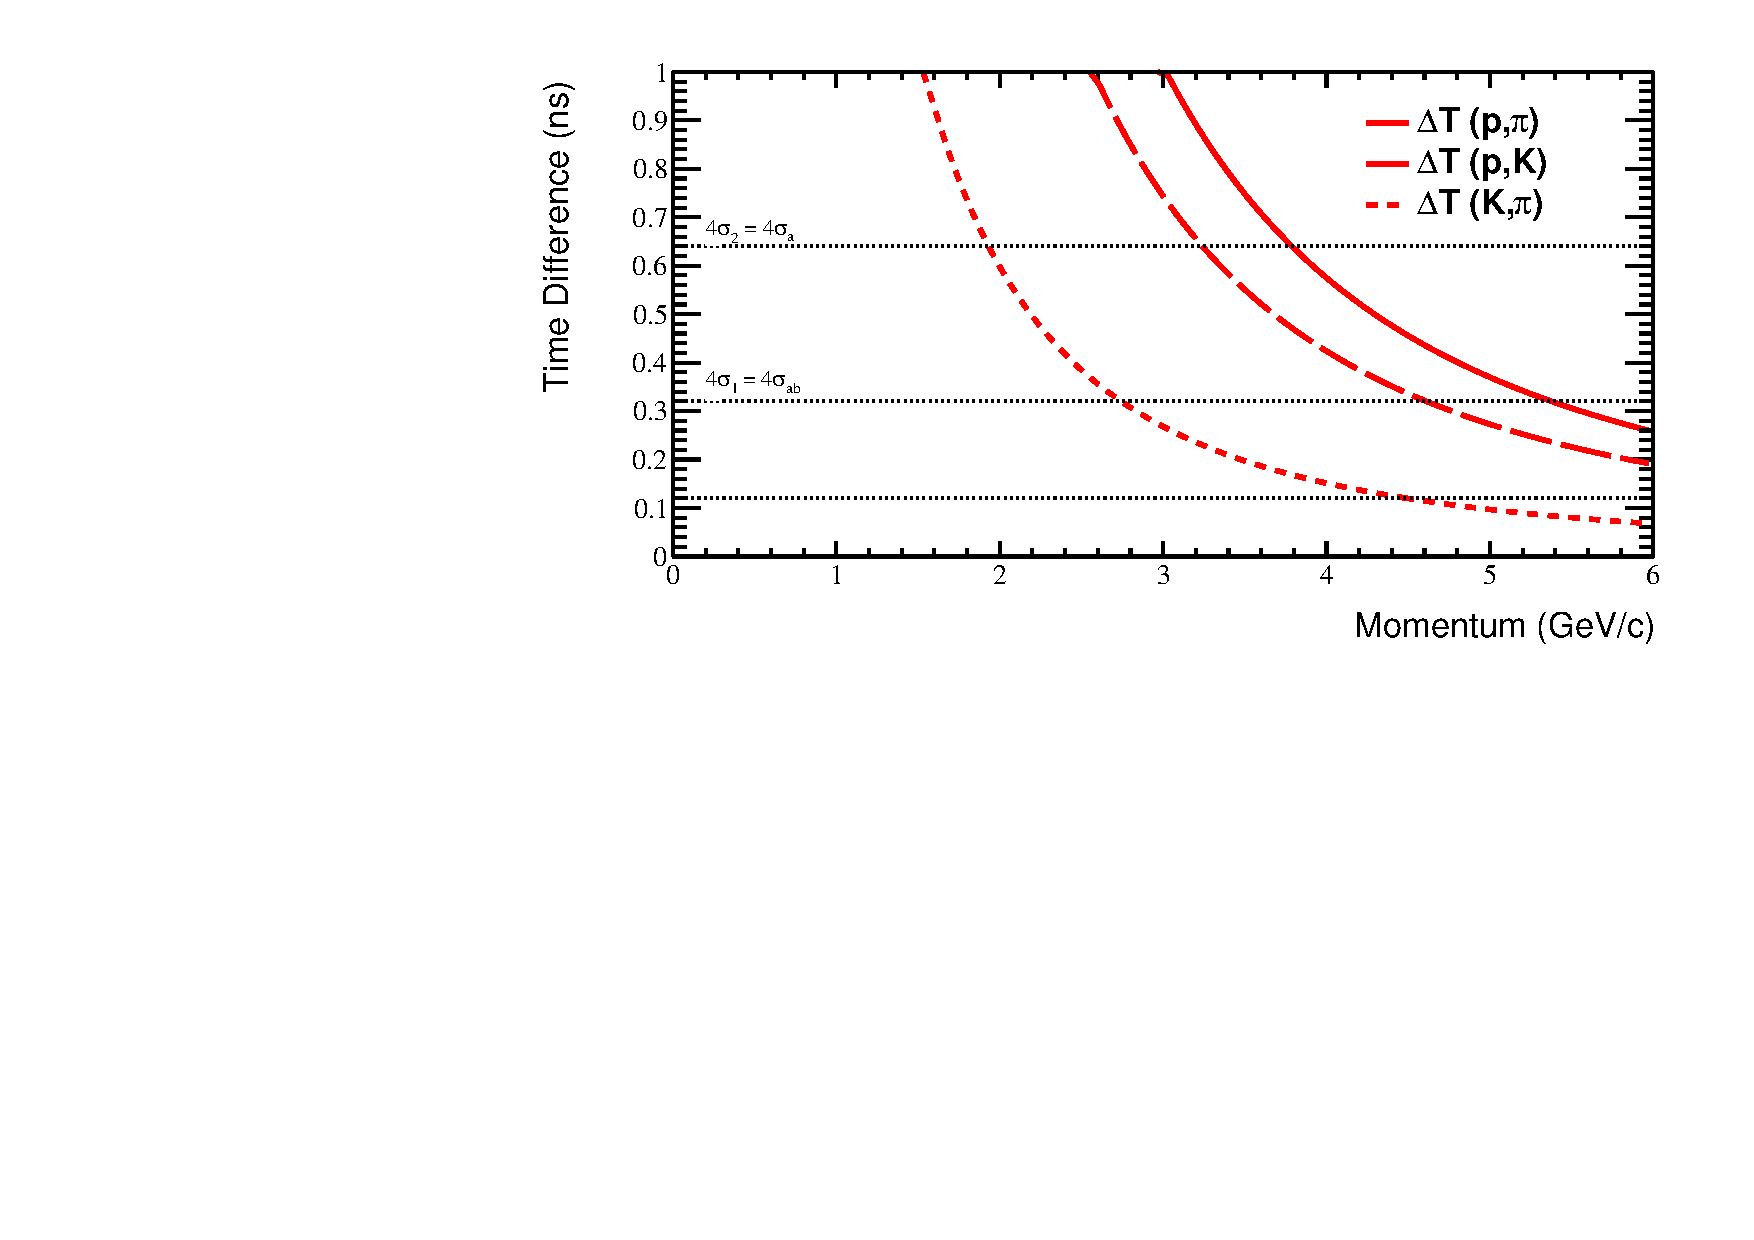
\includegraphics[width=6cm,height=6cm]{evan/fig_evan_ftof_requirements/DeltaT.pdf}}
\caption{The three curves indicate the time differences,$\Delta t$, between $p/\pi$,$p/K$, and $\pi/K$ over the $650\;cm$ path length from the target to Panel 1B. }
\label{fig:DeltaT}
\end{figure}
\begin{figure}[h!]
\centering
\mbox{\subfigure[$\:$Particle separation.]{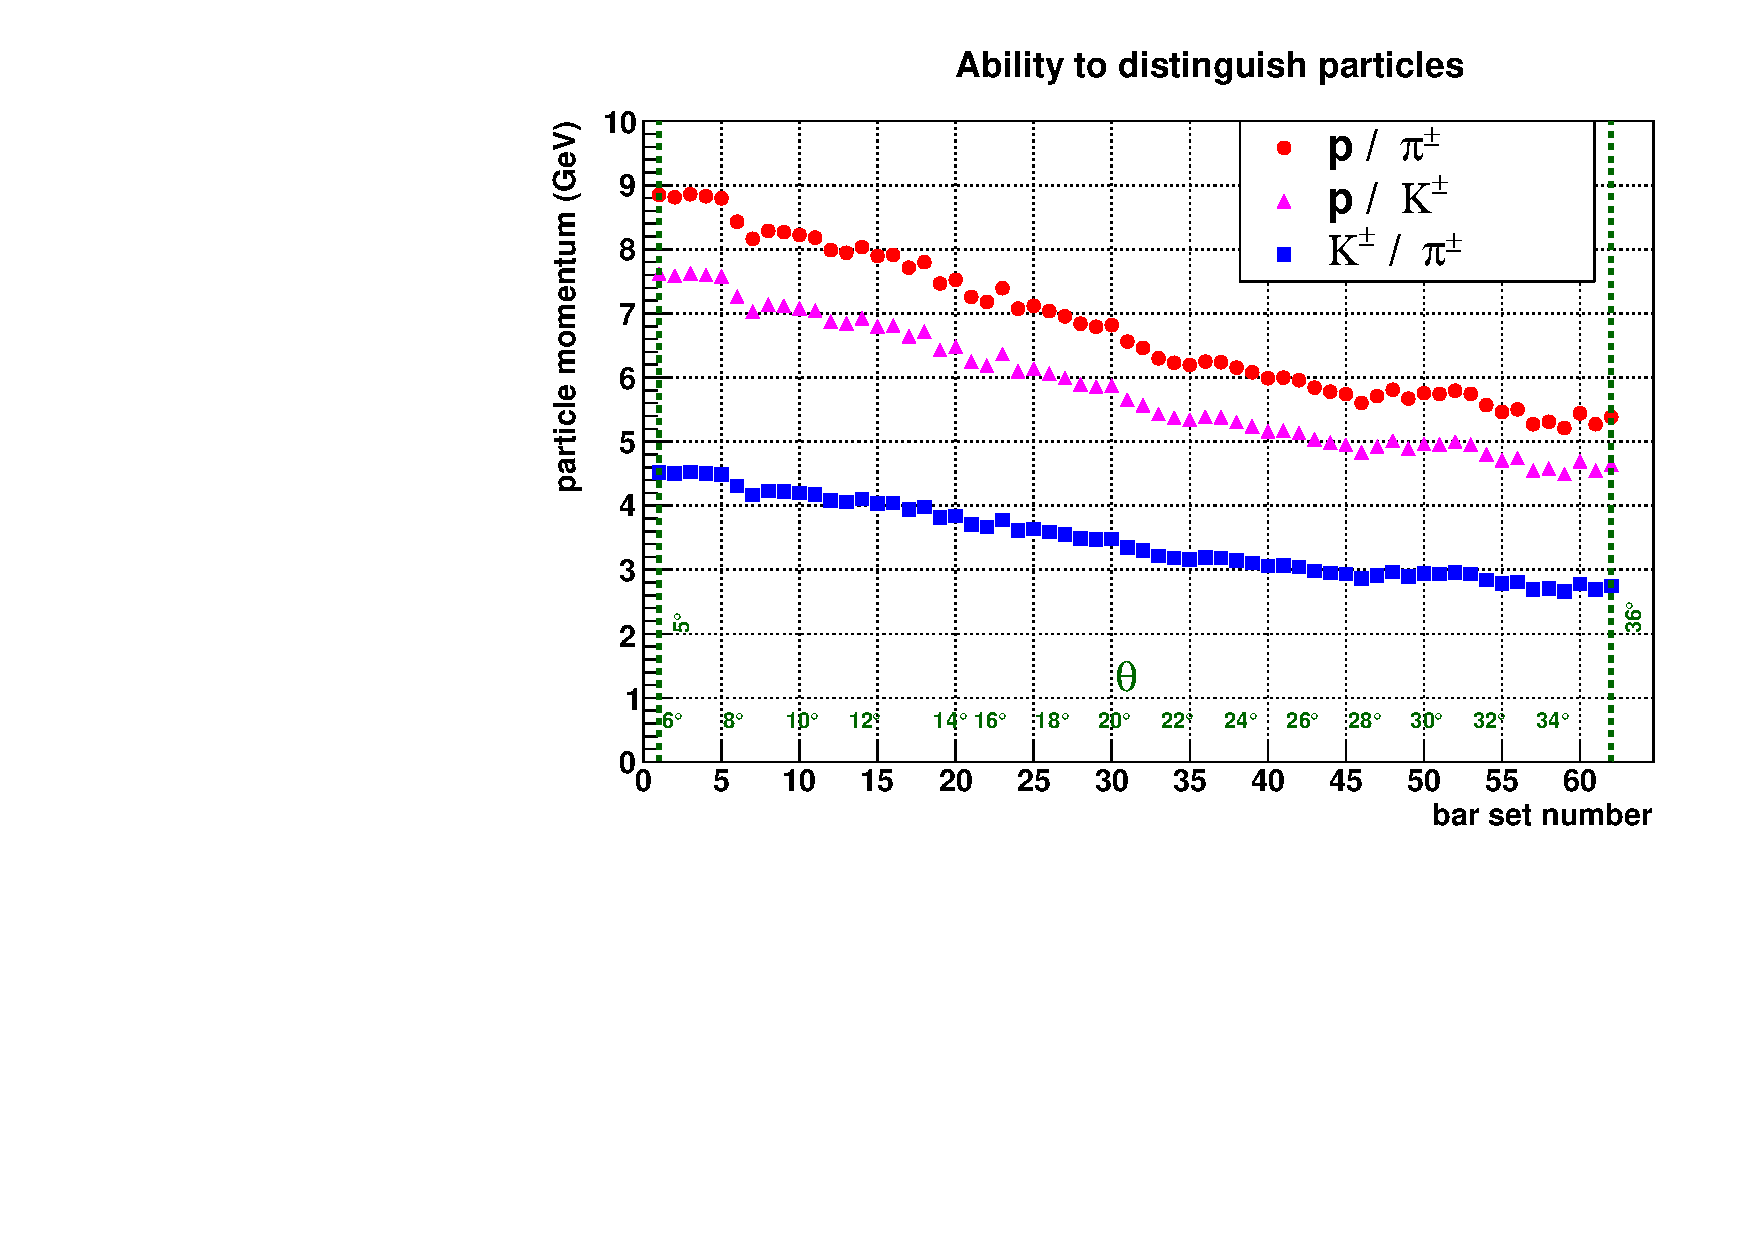
\includegraphics[width=0.4\textwidth]{evan/fig_evan_ftof_requirements/p_max.pdf}}\quad
\subfigure[$\:$Resolution curves.]{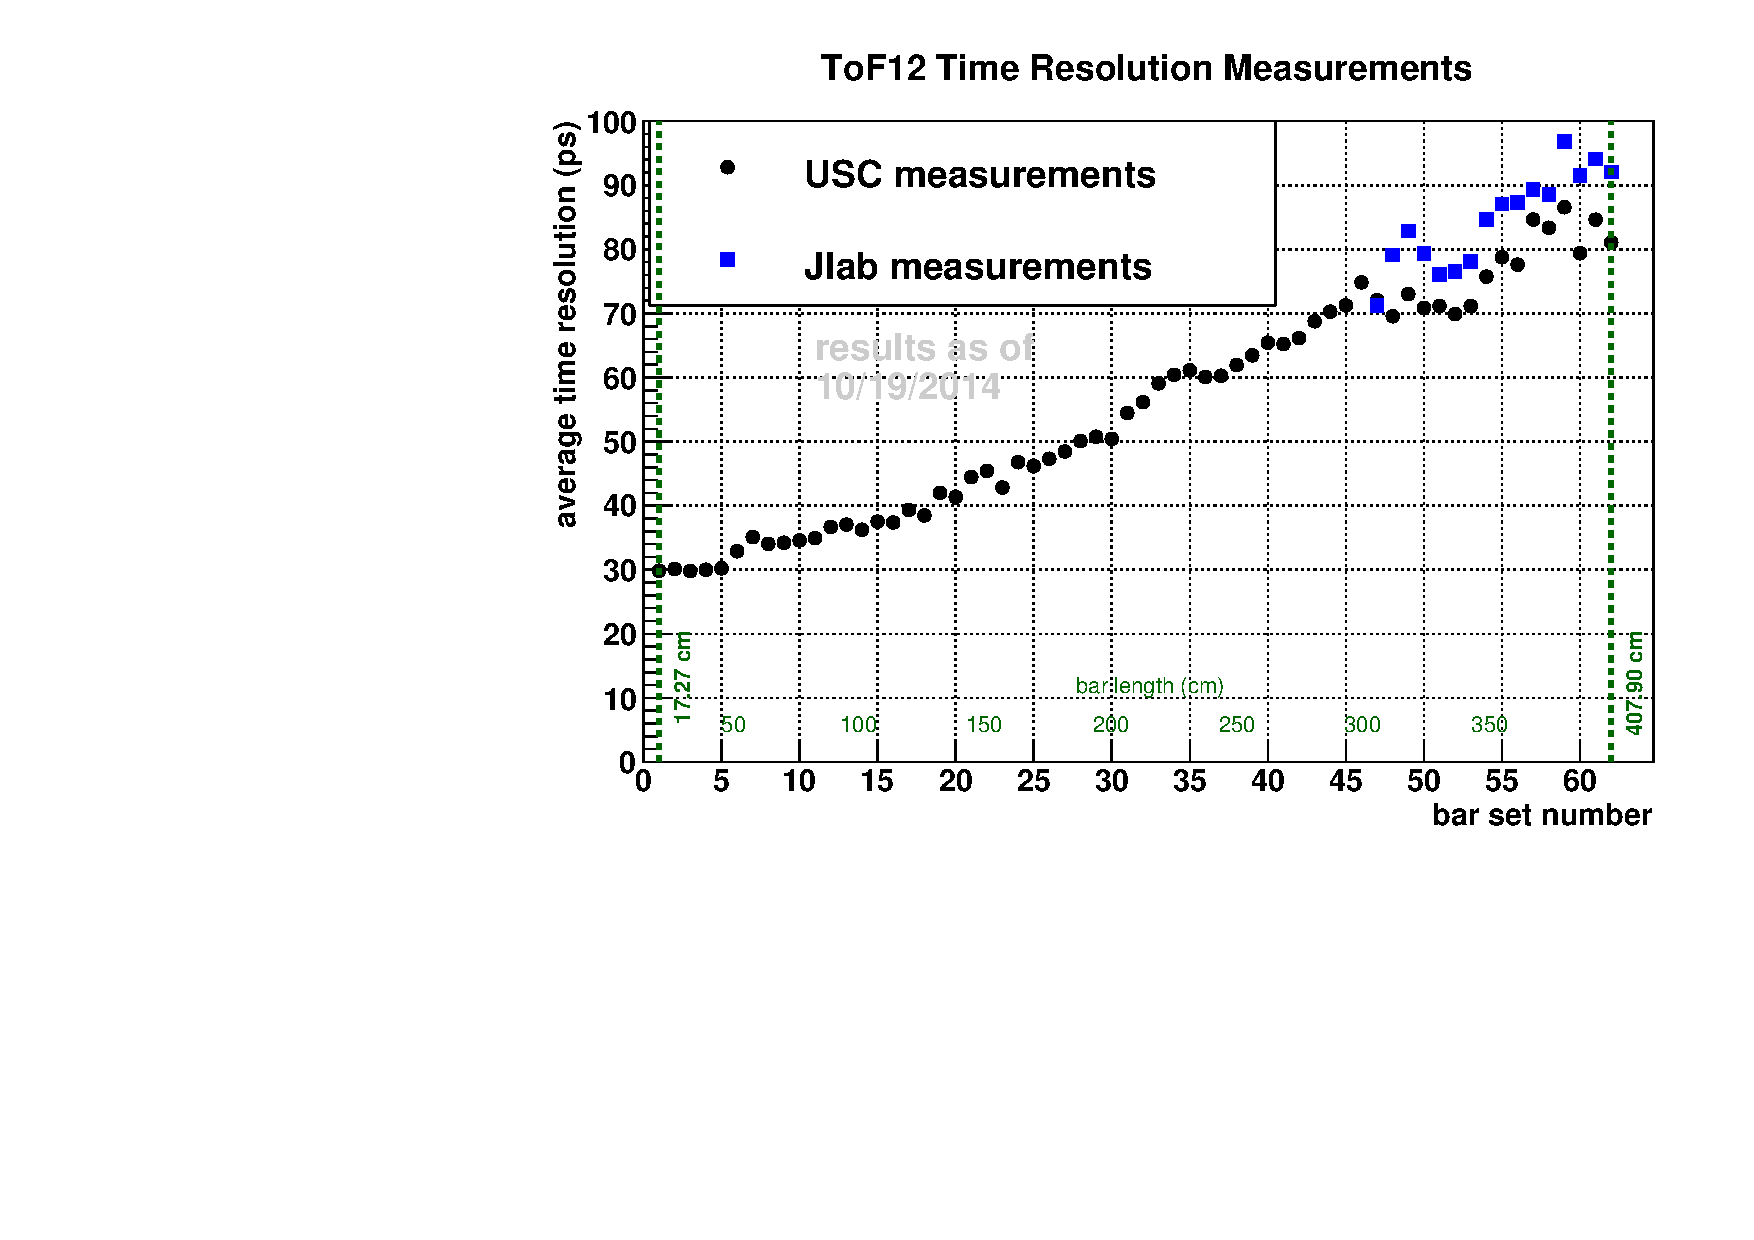
\includegraphics[width=0.4\textwidth]{evan/fig_evan_ftof_requirements/res.pdf}}}
\caption{(a) Maximum momentum up to which particles can be separated as function of bar set number or polar angle thete. Calculations were made in assumption of 650-$cm$ path length from the target to Panel 1B.~\cite{tdr}. Various symbols represent different particle pairs:  red circles - $p$/$\pi$, purple triangles - $p$/$K$, and  blue squares - $K$/$/pi$. (b) Average time resolution as function of bar set number or bar length. Black circles represent measurements performed at USC, while blue squares correspond to JLab measurements. For USC results resolutions of individual bars were averaged, while for JLab results resolution of three bar combinations were averaged. \label{fig:partIdReq}\label{fig:resLength}}
\end{figure}

As in the current $6$-$GeV$ FTOF detector (Panel 1A), each counter of the additional $12$-$GeV$ FTOF (Panel 1B) is composed of a long rectangular plastic scintillator with two cylindrical PMTs, one on each end, directly attached without light guides. The scintillator lengths are tightly constrained by the established six-panel FTOF geometry and the requirement that the new panels do not  restrict the CLAS12 acceptance as defined by the other detector components, but the thickness and width, $6\:cm \times 6\:cm$, are selected to optimize photon statistics, geometric matching with the photocathodes, and closest possible stacking. Compared to the Panel-1A $5\:cm \times 15\:cm$ FTOF scintillators, the $6\:cm \times 6\:cm$ scintillators increase the number of photons produced by a factor of 6/5; the increased ratio of photocathode area to scintillator exit window area increases the number of photons that reach the photocathode by at least a factor of 25/12.  Thus, disregarding that the area ratio factor acts on the number of photons after light attenuation, the Panel-1B scintillator geometry increases the number of photons reaching the photocathode by a factor of about 5/2 and, therefore, improves the resolution by a factor of $\sqrt{2/5}$, neglecting the resolution of any contributions that are independent of light level.

With a resolution of better than $150\:ps$ for the longest counters of Panel 1A, the Panel-1B counters must achieve resolutions better than $95\:ps$ for the combined resolution goal of $80\:ps$ to be reached (Fig.$\:$\ref{fig:resLength}). Preliminary prototype results exceed this requirement.
